
\chapter{基于改进的RetianNet骨髓血细胞检测网络}
\section{引言}

第三章中,我们对比了多个单阶段与双阶段检测网络在骨髓血细胞数据上的性能,综合考虑计算量,参数量与检测精度等因素,
我们选择将性能优异的RetinaNet作为基线模型。此外我们确定了先检测再识别的骨髓血细胞处理流程,即检测网络只需要进行
对血细胞进行前景检测与坐标回归。在RetianNet基线模型中,尽管模型的检测精度已经很高,但仍然存在着漏检、密集与重叠的血细胞区域
边界检测错误等问题,如图~\ref{fig:detect_problem}所示。

骨髓血细胞检测主要有如下三个难点:(1)相比外周血红细胞、白细胞、血小板三类血细胞检测,骨髓血细胞种类繁多、
形态丰富,尺寸大小不一。(2)在骨髓涂片制作过程中,由于染色剂与光照条件的变化,多个批次的数据存在着色彩差异。此外图像
背景复杂,存在较多成熟红细胞的干扰。(3)对于骨髓细胞增生活跃的切片,存在大量血细胞密集堆叠,边缘黏连,易导致漏检、错检等问题。
因此精准检测到骨髓血细胞是一项十分具有挑战性的课题。

针对上述难点与基线模型中存在的问题,本章提出了一种改进RetinaNet网络。该方法中,我们提出了一种基于全局注意力的自底向上的路径聚合网络结构,
缩短了底层与顶层特征之间的信息传递路径,提升网络对位置特征的提取能力。此外探究了不同标签分配策略对检测性能的影响,
提出基于最优输运的标签策略用于密集区域的血细胞的标签分配,避免了模糊分配样本的出现,提高网络对血细胞的召回能力。
最后我们比较了空洞卷积、深度可分离卷积、可变形卷积等卷积网络,以期实现速度与检测精度的更优平衡。
在骨髓血细胞数据集上的实验结果表明,本文提出的改进方法在检测准确率上有较大的提升,达到了较为先进的性能。

\begin{figure}[htbp]                     
  \centering                      
  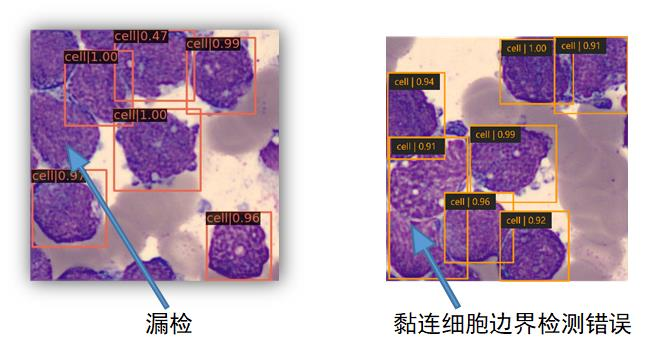
\includegraphics[width=0.65\linewidth]{detect_problem.jpg}                      
  \caption{RetinaNet基线模型检测错误示例}                      
  \label{fig:detect_problem}       
\end{figure}  

\section{改进的RetinaNet骨髓血细胞检测网络}
本章提出的改进RetinaNet网络结构如图~\ref{fig:improved_retinanet}所示,网络的输入是多张骨髓血细胞图像,大小为
$B \times 3 \times H \times W$。整个网络结构在第三章的RetinaNet基线模型进行改进。骨干网络为
ResNet50用于图像特征提取,特征金字塔结构用于多尺度特征提取。锚框的尺寸、数量与分类回归网络结果与基线模型相同。
为了提高网络检测的精度,我们在特征金字塔后引入了自底向上的路径聚合模块,该模块基于全局注意力将更浅层的特征与FPN深层的进行融合,
提升网络定位特征的表达能力,此外我们引入了可变形卷积、空洞卷积等卷积模块。在训练过程中,我们使用基于最优输运的策略进行标签分配。
下面各个小节将详细介绍我们的改进点。
\begin{figure}[htbp]                     
  \centering                      
  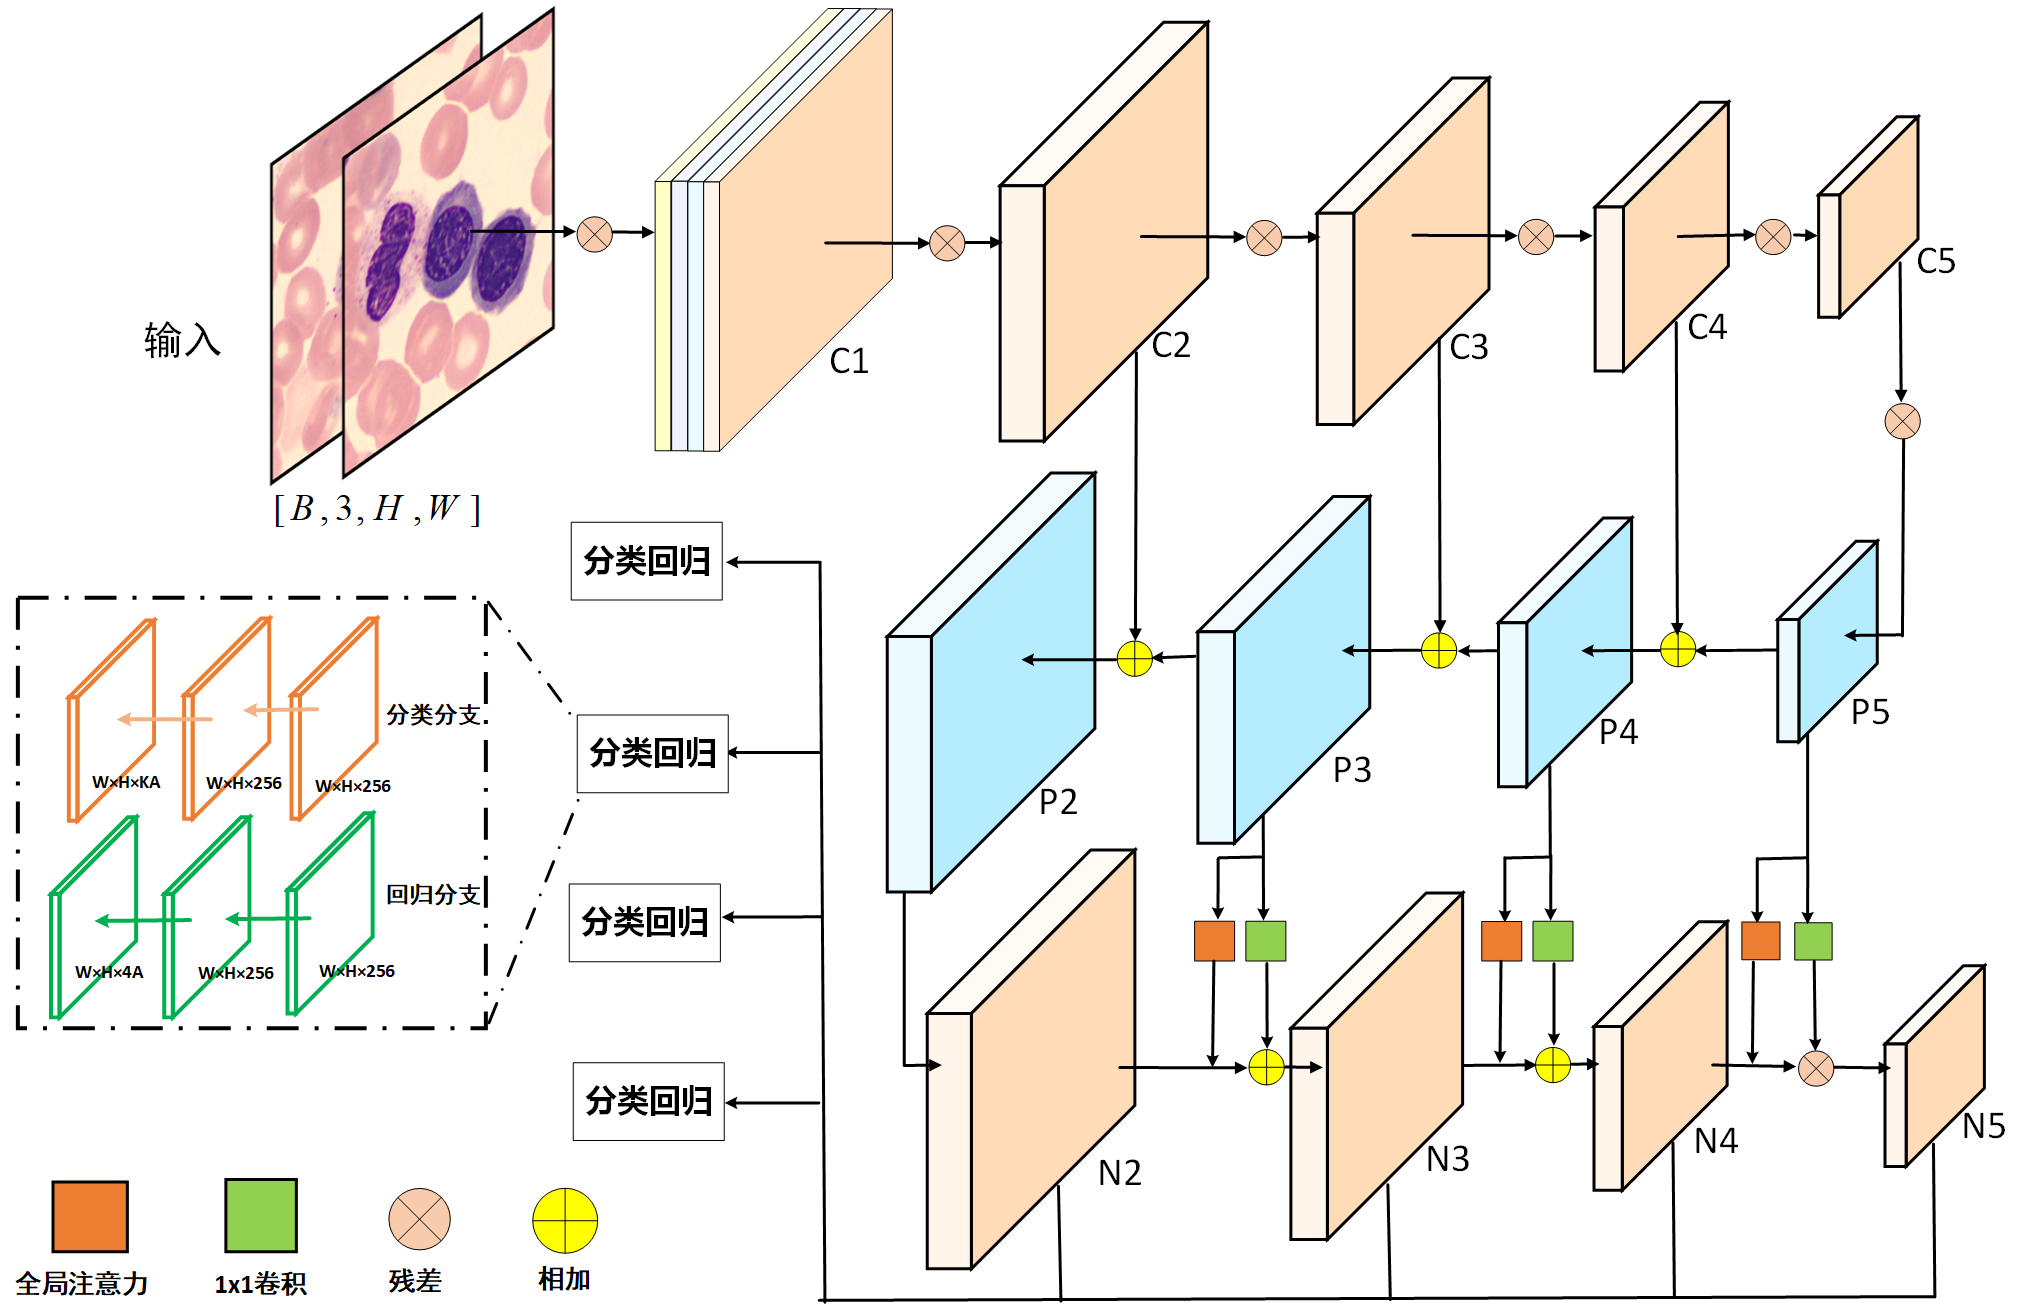
\includegraphics[width=0.95\linewidth]{improved_retinanet.png}                      
  \caption{RetinaNet基线模型检测错误示例}                      
  \label{fig:improved_retinanet}       
\end{figure}  

\subsection{基于全局注意的路径聚合网络}
\subsection{卷积模块}
\subsection{训练标签分配策略}

\section{算法实现与实验结果分析}
\subsection{实验环境}
\subsubsection{数据集介绍}

骨髓血细胞图像来自邃蓝智能科技(上海)有限公司合作医院提供,首先采用第2.1小节阐述的主动学习标注策略进行边界框的标注。
我们总共标记了6821张血细胞图像,训练集与测试集按照4:1的比例进行随机划分,训练集包含了5456张图像,测试集包含了1365张图像。
通常每个图像中包含1到10个有核血细胞,数据集总共标记了11352个血细胞,训练集有9065个血细胞,测试集有2287个血细胞。数据集的分布如
表~\ref{table:cell_detect1}所示:

\begin{table}
  \caption{骨髓血细胞检测数据集分布}   
  \centering 
  \label{table:cell_detect1}
  \begin{tabular}{ccccc}
    \toprule[2pt]
    序号 & 类别名  &  类别简写 & 训练集数量 & 测试集数量 \\
    \midrule[1.5pt] 
    1 & 原始细胞 & Prim & 1856 & 467 \\ 
    2 & 淋巴细胞 & Lym & 996 & 226   \\ 
    3 & 单核细胞 & Mono & 206 & 52   \\ 
    4 & 浆细胞 & Plas & 272 & 70   \\ 
    5 & 红细胞 & Red & 1880 & 503   \\ 
    6 & 早幼粒细胞 & Promy & 357 & 107   \\ 
    7 & 嗜中性中幼粒细胞 & Myelo & 701 & 150   \\ 
    8 & 嗜中性晚幼粒细胞 & Late & 503 & 144   \\ 
    9 & 嗜中性杆状核细胞 & Rods & 998 & 241   \\  
    10 & 嗜中分叶核细胞 & Lobu & 821 & 195   \\  
    11 & 嗜酸性粒细胞 & Eosl & 475 & 132   \\  
    \hline
    总计 &   &   & 9065 & 2287 \\
    \bottomrule[2pt]      
  \end{tabular} 
\end{table}


\subsection{实验结果与分析}
\subsubsection{评价指标} 
\subsubsection{实验结果}
\subsubsection{路径聚合网络}
\subsubsection{标签分配策略}
\subsubsection{不同卷积模块对实验结果影响}
\section{小结}


